\chapter{Evaluation}
\label{ch:evaluation}

% OK

Perhaps the most important part of a creative system is evaluation, both internally as external.
This chapter goes over both.
Due to the limited resources, internal evaluation is non-optimal but solutions are proposed.
Some of the reoccurring issues with the system's output are also discussed.
A heavy focus was put on the external evaluation and a custom build evaluation tool was made.
How this tool works and the results of the external evaluation are discussed here.

%------------------------------------
\section{Internal evaluation}
\label{sec:internal_evaluation}

As was already discussed, the discriminator is responsible for automatic internal evaluation.
The generator can use it to assess the quality of the generated image by either being accepted as real or not.
However, the point was raised that it is not possible to validate whether the generated images differ enough from existing cars.
If the discriminator is too strict, the generator can end up generating nearly identical images to the one in the training set.
Such a system would produce incredibly realistic results but is hard to call creative.
Currently, StyleGAN2 and other state-of-the-art models don't seem to have a metric in place to strictly evaluate this behaviour.

However, as was already discussed, a solution for this problem exists in the form of a reverse image search analysis.
Due to limited resources for this paper, this was not implemented.
However, the documentation on where the generation of new images occurs in the extended GANSpace tool is discussed.
This allows for future extensions where an automatic evaluator can be made to skip the output of the StyleGAN2 model that resembles a car from the training set too much.
It is noted that this ideology was used in the selection of images for evaluation, where three domain experts sat together to discuss which cars they recognized.
These experts were a Peugeot car mechanic, a Mercedes sales manager and a Honda employee. 
From this, a selection similar to the use of such an evaluation metric was made.
It is also important to note that providing this metric inside GANSpace would make it a wrapper function, meaning, the actual training of the model remains unchanged.
In an ideal world, this evaluation metric would be built into the used GAN technology.

Finally, the extended GANSpace tool helped validate the GAN has indeed learned concepts related to car design by using the same reasoning as the discussed paper by \citet{invidualunitanalysis}.
The generation process thus consists of making an image that contains learned concepts of a car.
Since the generated car designs are different enough from existing cars, they can be deemed creative in a similar manner \citet{creativecargan} deemed their system creative.



%------------------------------------
\section{Challenges for the GAN}
\label{sec:challenging_angle}

\begin{figure*}
\centering
\begin{subfigure}{.3\textwidth}
  \centering
  \includegraphics[width=\textwidth]{images/double_front.png}
  \caption{Double front car}
  \label{fig:doublefront}
\end{subfigure}%
\hspace{.02\textwidth}
\begin{subfigure}{.3\textwidth}
  \centering
  \includegraphics[width=\textwidth]{images/missing_piece.png}
  \caption{Missing piece in bed}
  \label{fig:missingpiece}
\end{subfigure}
\hspace{.02\textwidth}
\begin{subfigure}{.3\textwidth}
  \centering
  \includegraphics[width=\textwidth]{images/text.png}
  \caption{Attempt at text}
  \label{fig:textattempt}
\end{subfigure}
\captionsetup{width=.85\linewidth}
\captionsetup{justification=centering}
\caption{Multiple images generated by the system that demonstrate some of its flaws. Settings and more info available on GitHub \citep{github_project}.}
\label{fig:challanging_angle}
\end{figure*}

Whilst analysing the output of the GAN, it became visible the GAN had some reoccurring issues with its generated images.
One of these issues is what the documentation available on GitHub calls the 'challenging' angle.
When looking at the car from an angle in between front and side, the GAN seems to confuse what is front and back.
This results in realistic images of cars that have two fronts or two backs.
One such example is shown in figure \ref{fig:doublefront}.

Another challenge seemed to be that the GAN didn't always seem to generate the car in all dimensions.
This is shown in figure \ref{fig:missingpiece}, where a piece of the bed on the pick-up and convertible crossover is missing and replaced by grass.
Including images where such dimensions are missing might be interesting for the external evaluation to get an idea if participants notice it. 

The final reoccurring issue that is worth mentioning, is the system's poor performance in generating realistic backgrounds.
Whilst generating static backgrounds such as grass and trees was pretty successful most of the time, generating more complex environments often failed.
It could be argued this is a good thing, as it means the discriminator and generator have a focus on the realism of the car, which is the purpose of this system.
One of the most interesting phenomenons with background generation was the system's attempt at generating text.
An interesting example of this is shown in figure \ref{fig:textattempt}.

Other reoccurring anomalies from regular car designs were also noticed.
One such example is the fact that the headlight design was different on the other side of the car.
Whilst this is (almost) never found in car designs presents, it's not seen as an "issue of the GAN".
Besides this, the generated cars are often relatively symmetrical.
It is noted that the GAN also produced some outlandish results from time to time.
However, this was less than 10\% over more than 500 samples.
One such artefact is shown in figure \ref{fig:survey_creative_artefact}.



%------------------------------------
\clearpage
\section{Making a suitable external evaluation tool}
\label{sec:external_evaluation_tool}

\begin{figure*}
\centering
\begin{subfigure}{.3\textwidth}
  \centering
  \includegraphics[width=\textwidth]{images/survey1.PNG}
  \caption{Explanation of survey}
  \label{fig:explain_survey}
\end{subfigure}%
\hspace{.02\textwidth}
\begin{subfigure}{.3\textwidth}
  \centering
  \includegraphics[width=\textwidth]{images/survey2.PNG}
  \caption{Personal information}
  \label{fig:personal_info_survey}
\end{subfigure}
\hspace{.02\textwidth}
\begin{subfigure}{.3\textwidth}
  \centering
  \includegraphics[width=\textwidth]{images/survey3.PNG}
  \caption{Single image rating}
  \label{fig:single_survey}
\end{subfigure}
\captionsetup{width=.85\linewidth}
\captionsetup{justification=centering}
\caption{Screenshots of the created external evaluation tool.}
\label{fig:survey}
\end{figure*}


This paper aimed to make a creative system capable of generating photorealistic novel car designs.
The external evaluation helps in proving this goal is reached.
To ensure proper evaluation, a custom made PHP based survey tool is made.
This tool is based on a previous project from the author of this paper \citep{bapproef}.
Some screenshots of the tool, which was made available online\footnote{\url{https://www.lennertbontinck.com/creative-car-design-survey/}}, are shown in figure \ref{fig:survey}.
The flow of the system is described below.
\begin{itemize}
    \item Initialize the evaluation tool by visiting setup.php using the chosen key. This will create all required SQL tables and insert the images from the images folder into the images table. This step has to be performed only once.
    \item Participants can now complete the survey by navigating to the index.php web page.
    \item Show participant what personal information will be collected and what the survey is about.
    \item Show a more detailed explanation of all fields that need answering (see figure \ref{fig:explain_survey}):
    \begin{itemize}
        \item Explains some images are made by a computer algorithm and others by a human through photo editing software.
        \item Explains the backgrounds and logos have been tampered with on purpose to make the above choice harder. This is done due to the issues the GAN has with more complex backgrounds as described earlier.
    \end{itemize}
    \item Ask the user some personal information (see figure \ref{fig:personal_info_survey}):
    \begin{itemize}
        \item Gender (optional) and age in multiple of 10. The latter is done to improve anonymity. 
        \item Expertise: Participant is considered to have expertise in the domain if he is capable of recognizing cars from different brands from any angle.
        \item Whether the participant is colour blind or has other vision issues when taking the survey (e.g. not wearing glasses).
    \end{itemize}
    \clearpage
    \item Show two grouped images and four single images. These are selected at random from the evaluation set.
    \begin{itemize}
        \item Grouped images are images where the GANSpace tool is used to perform modifications. The following criteria are asked using a Likert scale from one to five:
        \begin{itemize}
            \item Correspondence: an image is considered of good correspondence (5) if the cars displayed in the row "start" are recognisable in the variants displayed below and modifications performed are similar between all four cars.
            \item Realism: an image is considered very realistic (5) if it could be an image from a car magazine.
            \item Creativity: Subjective measure, recognition of (elements of) existing cars can influence this.
            \item Made by: Whether participant thinks the modifications are made by a human or a computer.
            \item Notes: field for the participant to leave notes such as recognized cars.
        \end{itemize}
        \item Single images are images straight out of the StyleGAN2 model, taking into account the selection done using the similarity measure. The following criteria are asked using a Likert scale from one to five:
        \begin{itemize}
            \item Car: how "car-like" the object shown is, does it have all required components etc.
            \item Detail: a detailed image (5) contains minor details such as small badges, door handles, dents, reflections, ... If the image is rather "flat", it would receive a lower score.
            \item Realism: same ideology as before.
            \item Resemblance: an image is considered very resemblant (5) of another car if the participant recognizes a certain existing car in the image. It's loosely resemblant (3) if he recognizes the style treats of a car or brand.
            \item Creativity: same ideology as before.
            \item General impression: how the participant would rate this image in general.
            \item Made by: same ideology as before.
            \item Notes: same ideology as before.
        \end{itemize}
    \end{itemize}
    \item Show the participant a screen admitting he's been lied to and all images have been computer-generated. Ask whether or not the participant thinks he was biased.
    \item Similarly show the other evaluation images. The "made by" field is now automatically set to "known".
    \item Export all SQL tables to CSV files by navigating to the export.php web page using the chosen key.
\end{itemize}

The tool is made available under the GPL V3 license and is available with documentation on the GitHub repository of this project \citep{github_project}.
On the same GitHub page, all used images for the external evaluation and the documentation to reproduce them is also available.
Some of the images generated through GANSpace modifications were minor changes such as different wheel designs whilst others were major changes such as making a car look more sporty.
These are displayed in figure \ref{fig:groupedsurvey}.
The single images contained various examples, from super realistic examples to creative artefacts of the system.
Some are shown in figure \ref{fig:singlesurvey}.


\begin{figure*}
\centering
\begin{subfigure}{.3\textwidth}
  \centering
  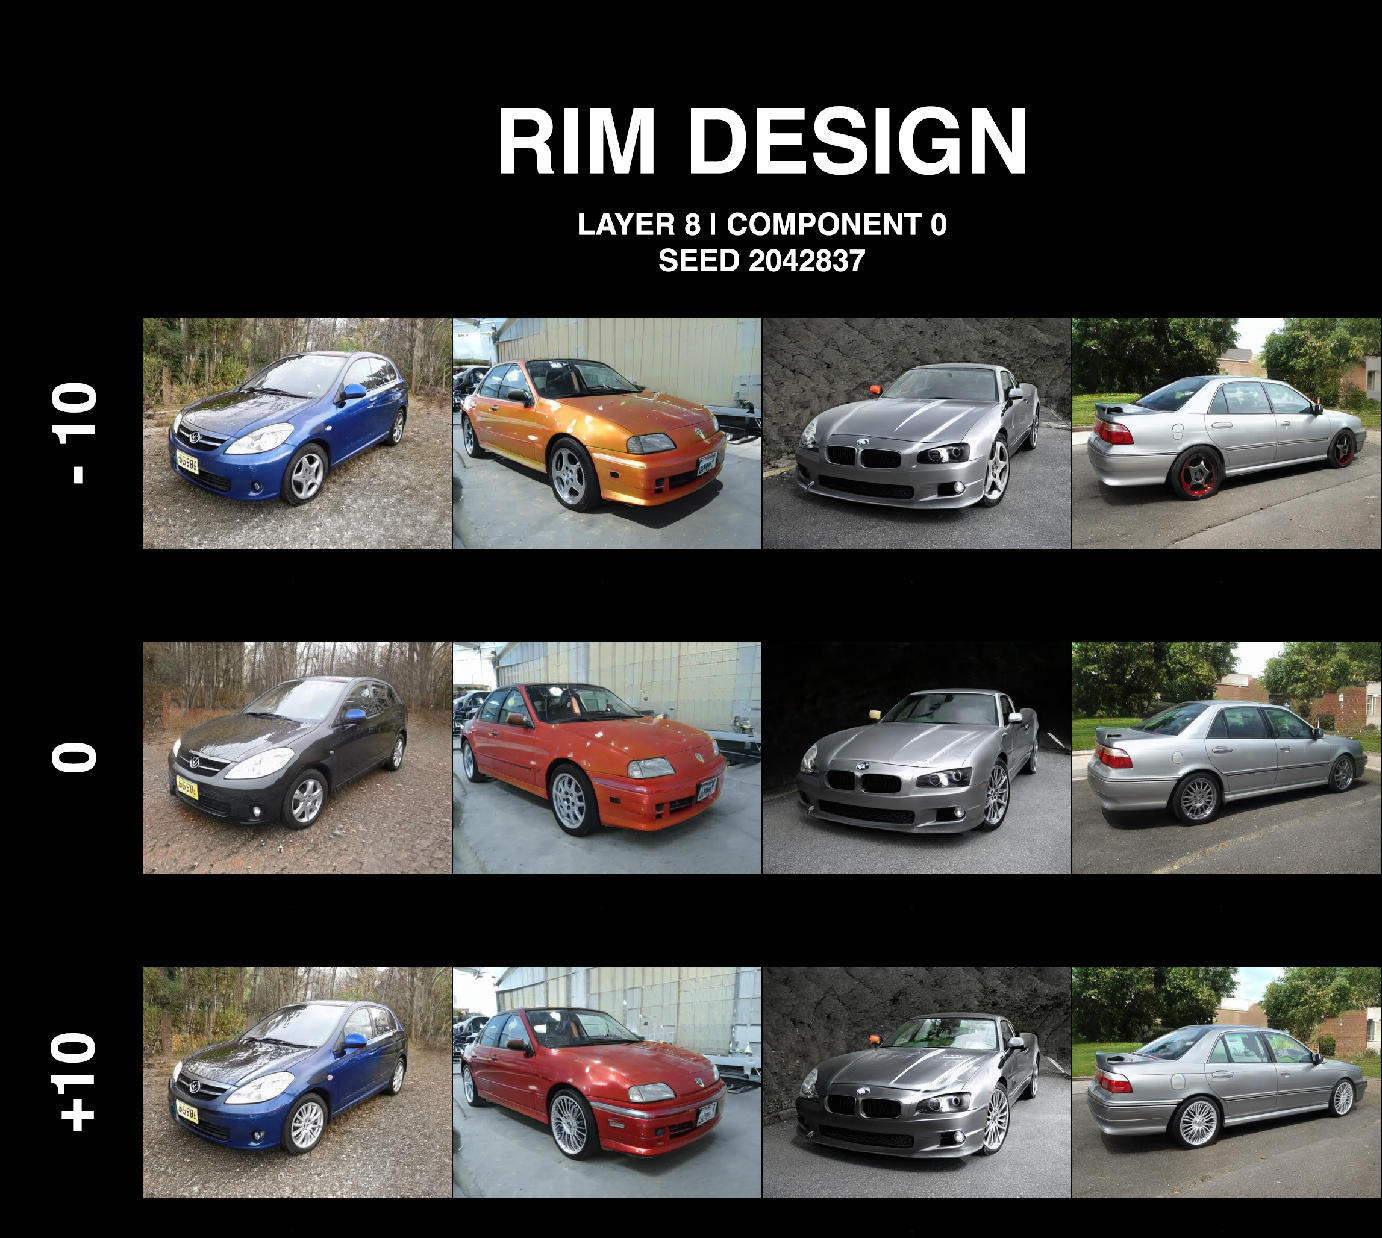
\includegraphics[width=\textwidth]{images/rim_design.pdf}
  \caption{Minor edits}
  \label{fig:rimdesign}
\end{subfigure}%
\hspace{.02\textwidth}
\begin{subfigure}{.3\textwidth}
  \centering
  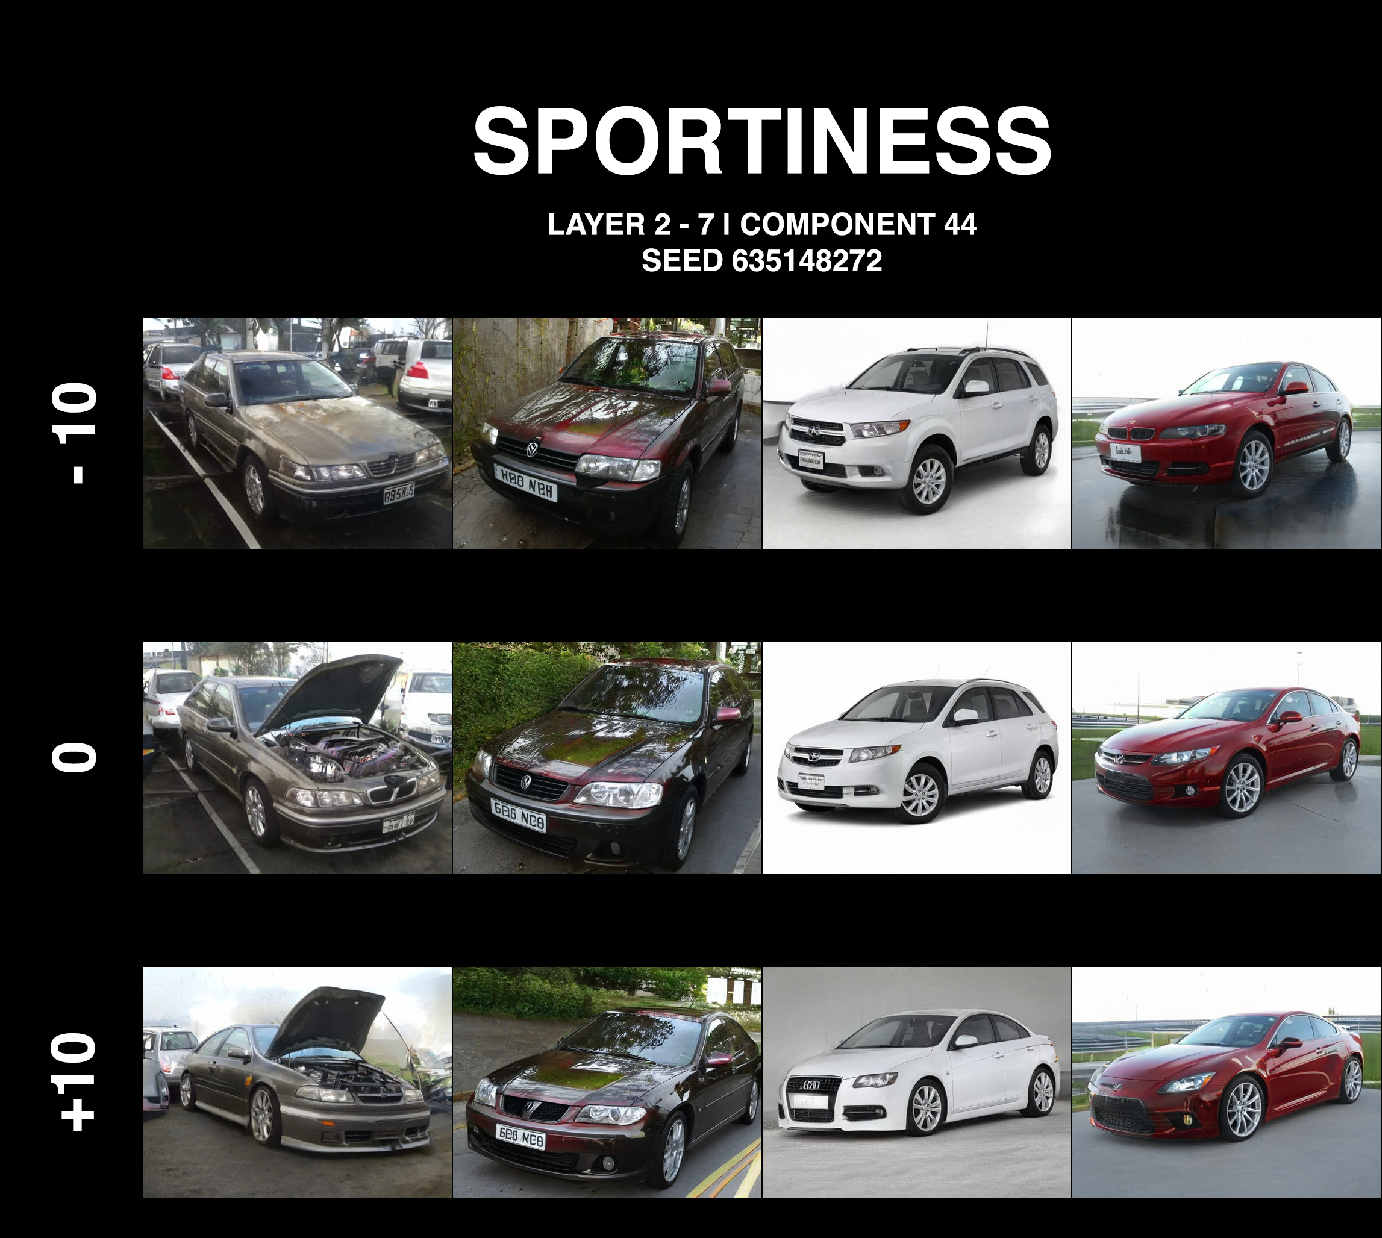
\includegraphics[width=\textwidth]{images/Sportiness.pdf}
  \caption{Major edits}
  \label{fig:sportiness}
\end{subfigure}
\hspace{.02\textwidth}
\begin{subfigure}{.3\textwidth}
  \centering
  \includegraphics[width=\textwidth]{images/flat_front.pdf}
  \caption{Major edits}
  \label{fig:flatfront}
\end{subfigure}
\captionsetup{width=.85\linewidth}
\captionsetup{justification=centering}
\caption{Some of the grouped images used for external evaluation. Note that the textual description was removed when shown to the participant.}
\label{fig:groupedsurvey}
\end{figure*}

\begin{figure*}
\centering
\begin{subfigure}{.3\textwidth}
  \centering
  \includegraphics[width=\textwidth]{images/single1.png}
  \caption{Creative artefact}
  \label{fig:survey_creative_artefact}
\end{subfigure}%
\hspace{.02\textwidth}
\begin{subfigure}{.3\textwidth}
  \centering
  \includegraphics[width=\textwidth]{images/single6.png}
  \caption{Very realistic}
  \label{fig:survey_realistic}
\end{subfigure}
\hspace{.02\textwidth}
\begin{subfigure}{.3\textwidth}
  \centering
  \includegraphics[width=\textwidth]{images/single8.png}
  \caption{Challenging angle}
  \label{fig:survey_angle}
\end{subfigure}

\vspace{.02\textwidth}

\begin{subfigure}{.3\textwidth}
  \centering
  \includegraphics[width=\textwidth]{images/single2.png}
  \caption{Double front}
  \label{fig:survey_doublefront}
\end{subfigure}%
\hspace{.02\textwidth}
\begin{subfigure}{.3\textwidth}
  \centering
  \includegraphics[width=\textwidth]{images/single3.png}
  \caption{Missing piece}
  \label{fig:survey_missing}
\end{subfigure}
\hspace{.02\textwidth}
\begin{subfigure}{.3\textwidth}
  \centering
  \includegraphics[width=\textwidth]{images/single4.png}
  \caption{Mercedes/BMW merge}
  \label{fig:survey_merged}
\end{subfigure}
\captionsetup{width=.85\linewidth}
\captionsetup{justification=centering}
\caption{Some of the single images used for external evaluation.}
\label{fig:singlesurvey}
\end{figure*}



%------------------------------------
\clearpage
\section{External evaluation results}
\label{sec:external_evaluation_results}

The external evaluation contains a lot of distinct rating criteria.
Since it wouldn't be feasible to analyse all of the results here, a Jupyter Notebook doing a complete analysis is made available under the results folder on the GitHub repository of this project \citep{github_project}.
Since the survey was quite lengthy and there were some minor bugs early on, it was expected not all of the participants registered completed the survey.
Indeed, after removing non-complete entrees the list of participants shrank from 32 to 21.
Of those 21 participants, 16 were male and 5 were female.
There were 7 participants with expertise, all of which were male.
Most of the participants belonged to the 20 years age group, one was colourblind and none had other vision problems.
These distributions seem healthy for a topic that is known to have more interest by men.

The Notebook then analyses the distribution of the creator assignments for each image.
The data shows that the random selection was successful and some images were highly assigned to either human or computer made.
Single images that were highly assigned to computer-generated were those containing non-realistic designs such as the one shown in figure \ref{fig:survey_creative_artefact} and \ref{fig:survey_angle}.
Interestingly enough, the grouped images that were highly assigned to computer-generated were those that contained minor edits such as the rim design edit shown in figure \ref{fig:rimdesign}.
This is interesting since those minor edits are harder for GANs, as they require the knowledge of smaller concepts from a car's design such as the wheel design.
The more realistic single images such as the one shown in figure \ref{fig:survey_realistic} were highly assigned to human-made.
For the grouped images, the major edits such as the one shown in figure \ref{fig:sportiness} were highly assigned to human-made as well.

\begin{figure*}
\centering
\begin{subfigure}{.45\textwidth}
  \centering
  \includegraphics[width=\textwidth]{images/grouped_images_score_bias.png}
  \caption{Grouped image bias analysis}
  \label{fig:grouped_bias}
\end{subfigure}%
\hspace{.02\textwidth}
\begin{subfigure}{.45\textwidth}
  \centering
  \includegraphics[width=\textwidth]{images/single_images_score_bias.png}
  \caption{Single image bias analysis}
  \label{fig:single_bias}
\end{subfigure}
\captionsetup{width=.85\linewidth}
\captionsetup{justification=centering}
\caption{ Bias analysis of grouped and single images. Analysis on a per image basis available on GitHub in the results Jupyter Notebook \citep{github_project}. }
\label{fig:bias}
\end{figure*}

This initial look at the results hints that the participants were biased in assigning shocking designs and minor edits to computers whilst assigning high-quality design and major edits to humans.
To validate this, the assigned realism and creativity scores were analysed per image, grouped by the assumed origin of the picture.
These analytics revealed it was indeed the case scores of human thought design were higher for both realism and creativity than when they were assigned to computer-generated.
More surprising, it became clear that after knowing that all designs were made by computers, this negative bias towards computer-generated design got slightly less. 
It is noted that most of these differences are small and for some images not statistically significant.

Figure \ref{fig:bias} summarizes these bias findings by showing the average score and standard deviation for realism and creativity grouped per thought origin.
Whilst it is concluded from these results that a bias against computer-generated design is present, only 6 out of 21 participants thought they were biased.
Interesting notes on this included "[...] I might have assigned the broken looking ones to pc" and "[...] A few images were shockingly good. Very impressive stuff.".

\begin{figure*}
\centering
\begin{subfigure}{.45\textwidth}
  \centering
  \includegraphics[width=\textwidth]{images/text.png}
  \caption{Generated car}
  \label{fig:similarcar_gan}
\end{subfigure}%
\hspace{.02\textwidth}
\begin{subfigure}{.45\textwidth}
  \centering
  \includegraphics[width=\textwidth]{images/bentley-flying-spur.jpg}
  \caption{Bentley Flying Spur}
  \label{fig:similarcar_real}
\end{subfigure}
\captionsetup{width=.85\linewidth}
\captionsetup{justification=centering}
\caption{ Image of car generated by the GAN and the similar looking existing variant according to a participant. }
\label{fig:similarcar}
\end{figure*}

Since the notes from the bias gave an interesting insight into the participants' perception of the creative system, it was decided to have a look at the notes for the ratings similarly.
The most reoccurring notions from these notes are listed in what follows.
Be aware that these are generalisations of the received notes as no two notes are identical.
\begin{itemize}
    \item Notes that reoccurred on several images:
    \begin{itemize}
        \item "If it is computer-generated, it fooled me well."
        \item "[...] but weird artefact where [...]"
        \item "[...] these small changes make me give it a low creativity score." 
        \item "Reminds me of $<$car brand$>$."
        \item "[...] creative [...] not really a car [...]"
        \item "Don't really see a lot of difference." (grouped images with minor edits)
        \item "Look like completely different cars." (grouped images with major edits)
    \end{itemize}
    \clearpage
    \item Notes that reoccurred for specific grouped images:
    \begin{itemize}
        \item "[...] changed wheels [...]" (grouped image shown in figure \ref{fig:rimdesign})
        \item "[...] lowered [...] changed bumper [...] more sporty [...]" (grouped image shown in figure \ref{fig:sportiness})
        \item "[...] makes the car red [...]" (grouped image of flashy color modification)
        \item "[...] boxy [...] nose changes [...] (grouped image shown in figure \ref{fig:flatfront})
    \end{itemize}
    \item Notes that reoccurred for specific single images:
    \begin{itemize}
        \item "[...] looks nothing like a car [...] unique and creative [...] horror movie [...] album art [...]" (single image shown in figure \ref{fig:survey_creative_artefact})
        \item "[...] wow [...] interesting concept [...] weird thing with doors [...]" (single image shown in figure \ref{fig:missingpiece})
        \item "[...] Mercedes SUV [...] BMW headlights [...]" (single image shown in figure \ref{fig:survey_merged})
        \item "[...] cool text [...] Bentley Flying Spur [...]" (single image, comparison shown in figure \ref{fig:similarcar})
        \item "[...] funny [...] looks like another car drove into this one [...] seems confused about angles [...]" (single image shown in \ref{fig:survey_angle})
    \end{itemize}
\end{itemize}


\begin{figure*}
\centering
\begin{subfigure}{.45\textwidth}
  \centering
  \includegraphics[width=\textwidth]{images/creativity_minor_changes.png}
  \caption{Creativity for modifications}
  \label{fig:creative_minor_changes}
\end{subfigure}%
\hspace{.02\textwidth}
\begin{subfigure}{.45\textwidth}
  \centering
  \includegraphics[width=\textwidth]{images/single_images_creativity.png}
  \caption{Creativity for single images}
  \label{fig:creative_single_images}
\end{subfigure}
\captionsetup{width=.85\linewidth}
\captionsetup{justification=centering}
\caption{Creativity rating comparisons based on type of image. Data from participants that knew it was machine made.}
\label{fig:creativity_statistics}
\end{figure*}

These notes give a good insight into the impressions of the participants.
It becomes apparent that the found concepts through GANSpace were also recognized by the participants.
Whilst, as already discussed, the possibility of doing minor edits through GANSpace is technically more impressive, it seems to be less impressive and creative to participants.
This can also be seen in figure \ref{fig:creative_minor_changes} where the creativity rating for the color modification and sportiness modification from figure \ref{fig:sportiness} are compared.
This hints that the "shocking" aspect of creativity seems to play an important role in the participants' ratings.
Indeed, when doing a similar comparison between the unrealistic challenging angle (figure \ref{fig:survey_angle}), a basic merge (figure \ref{fig:survey_merged}) and a very realistic (figure \ref{fig:survey_realistic}) car design, the more shocking designs get better ratings than the typical looking car.
The Jupyter Notebook then goes further by looking at the correlation matrix and more.
These extra analysis steps are not reported further as they don't teach much new information.